\documentclass[11pt]{article}
\makeatletter\def\input@path{{../}}\makeatother
\usepackage{preamble}
\renewcommand{\chaptername}{Chapter 5: Hypothesis testing}
\graphicspath{{figures/}}

\begin{document}

\solutionstitlepage{5}{Hypothesis testing}{All numbers and figures are reproduced by \texttt{ch05/code/ch05.R} (base R + MASS).}

\tableofcontents
\clearpage

\section*{Answers at a glance}
\addcontentsline{toc}{section}{Answers at a glance}
\begin{center}
\small
\renewcommand{\arraystretch}{1.25}
\begin{tabular}{>{\bfseries\color{navy}}r p{0.82\linewidth}}\toprule
1 & $b=5.93\times10^{-4}$; BF $=2.4,\ 3.8,\ 10.1,\ 35.2$ --- never ``decisive'' ($>100$), strong only for $N\ge50$.\\
2 & $\log_{10}\text{BF}\approx42$ in favour of ``vaccine arm has the lower rate''; insensitive to the prior.\\
3 & BF(separate : common) $=1.40$ ($c=1$) but $0.14$ ($c=10$): the answer flips with the prior range.\\
4 & (a) $\Prob(\mu_1<\mu_2)=0.90$; (b) $\beta_2$ CI $(-1.8,\ 9.8)$; (c) $\Prob(\mu_1\neq\mu_2)=0.53\to0.13$ as $W$ grows.\\
5 & $\tau=1$: BF$>1$ iff $|y|>1.18$; $\tau=10$: iff $|y|>2.16$ (Lindley's paradox).\\
6 & Mean opens: A 0.96, B 2.02, C 1.06; $\Prob(\text{B best})\approx1$.\\
7 & Prior $\dist{Gamma}(0.44,\ 1359)$; BFDR 10\% gives $t=0.677$ and flags 8 regions.\\
8 & Type I error 0.050--0.084 ($>0.05$); power at $\lambda=1.5$: 0.53 ($n=10$) to 0.998 ($n=100$); randomise to get exactly 0.05.\\
9 & Most likely model drops \texttt{indus} and \texttt{age} (posterior probability 0.62).\\\bottomrule
\end{tabular}
\end{center}
\clearpage

% ================================================================= primer
\section*{A five-minute primer on the tools of this chapter}
\addcontentsline{toc}{section}{Primer: the tools of this chapter}

\begin{recall}
\textbf{1. Posterior probability of a hypothesis.} For hypotheses about a parameter (e.g.\ $H_1:\lambda\le1$ vs.\ $H_2:\lambda>1$), simply compute $\Prob(H_k\mid\mathbf Y)$ from the posterior.

\medskip
\textbf{2. Bayes factor.} For two hypotheses (or models),
\[
\text{BF}_{21}=\frac{\Prob(H_2\mid\mathbf Y)/\Prob(H_1\mid\mathbf Y)}{\Prob(H_2)/\Prob(H_1)}=\frac{\text{posterior odds}}{\text{prior odds}}=\frac{m_2(\mathbf Y)}{m_1(\mathbf Y)},
\]
where $m_k(\mathbf Y)=\int f(\mathbf Y\mid\theta,H_k)\pi(\theta\mid H_k)\dd\theta$ is the \emph{marginal likelihood} (how well $H_k$, averaged over its prior, predicted the data). With equal prior probabilities, posterior odds $=$ BF.

\medskip
\textbf{3. Interpreting a BF} (Jeffreys' scale): 1--3 barely worth mentioning, 3--10 substantial, 10--30 strong, 30--100 very strong, $>100$ decisive.

\medskip
\textbf{4. Sensitivity.} For a \emph{point} null ($\mu=0$) the BF depends strongly on how spread out the alternative's prior is: a very vague alternative spreads its prior mass thinly and is penalised (\textbf{Lindley's paradox}). One-sided tests are much less sensitive.

\medskip
\textbf{5. Multiple testing: Bayesian false discovery rate.} If we declare discoveries for all tests with $q_i=\Prob(\text{effect}_i\mid\mathbf Y)>t$, the expected proportion of false discoveries among them is
\[
\text{BFDR}(t)=\frac{\sum_i(1-q_i)\,\mathbb 1(q_i>t)}{\sum_i\mathbb 1(q_i>t)}.
\]
Choose the smallest $t$ with $\text{BFDR}(t)\le$ the target (e.g.\ 10\%).

\medskip
\textbf{6. Variable selection (SSVS).} Give each coefficient an inclusion indicator $\gamma_j\in\{0,1\}$; the posterior inclusion probability $\Prob(\gamma_j=1\mid\mathbf Y)$ measures the evidence that covariate $j$ belongs in the model.
\end{recall}

\clearpage

% ================================================================= Exercise 1
\exercise{5.1 --- A one-sided test for a Poisson rate}

\begin{problem}{1}
Assume that $Y|\lambda\sim\dist{Poisson}(N\lambda)$ and $\lambda\sim\dist{Gamma}(0.1,b)$. The null hypothesis is that $\lambda\le1$, and the alternative is that $\lambda>1$. Select $b$ so that the prior probability of the null hypothesis is 0.5. Using this prior, compute the posterior probability of the alternative hypothesis and the Bayes factor for the alternative relative to the null hypothesis for (a) $N=10$ and $Y=12$; (b) $N=20$ and $Y=24$; (c) $N=50$ and $Y=60$; (d) $N=100$ and $Y=120$. For which $N$ and $Y$ is there definitive evidence in favor of the alternative?
\end{problem}

\begin{restate}
The observed rate is always $Y/N=1.2$; only the amount of data grows. Choose a prior with median 1, then see how the evidence for $\lambda>1$ grows with $N$.
\end{restate}

\begin{recall}
\begin{itemize}
\item Poisson--gamma: $\lambda\mid Y\sim\dist{Gamma}(0.1+Y,\ b+N)$ (Chapter 2 primer).
\item \textbf{Scaling}: if $\lambda\sim\dist{Gamma}(a,b)$ then $b\lambda\sim\dist{Gamma}(a,1)$, so every quantile of $\lambda$ is the corresponding $\dist{Gamma}(a,1)$ quantile divided by $b$.
\end{itemize}
\end{recall}

\begin{keyidea}
Prior probability 0.5 for $\lambda\le1$ means the prior \emph{median} is 1. With equal prior odds, BF $=$ posterior odds.
\end{keyidea}

\solution
\step{Step 1 --- choose $b$.}
The median of $\dist{Gamma}(0.1,1)$ is $m=$ \texttt{qgamma(0.5, 0.1, 1)} $=5.934\times10^{-4}$. The median of $\lambda$ is $m/b$; setting it to 1 gives $b=m=5.93\times10^{-4}$.
\why{With shape 0.1 the Gamma is extremely skewed: most of its mass is near 0 but it has a very long tail, so its median is tiny on the $\dist{Gamma}(0.1,1)$ scale.}
\step{Step 2 --- posteriors.} $\lambda\mid Y\sim\dist{Gamma}(0.1+Y,\ 0.000593+N)$, so
$\Prob(H_2\mid Y)=\Prob(\lambda>1\mid Y)=$ \texttt{pgamma(1, 0.1 + Y, b + N, lower.tail = FALSE)}.
\step{Step 3 --- Bayes factors.} Prior odds $=0.5/0.5=1$, so $\text{BF}_{21}=\frac{\Prob(H_2\mid Y)}{1-\Prob(H_2\mid Y)}$.
\begin{center}
\begin{tabular}{ccccl}\toprule
 & $N$ & $Y$ & $\Prob(\lambda>1\mid Y)$ & $\text{BF}_{21}$ (Jeffreys' scale)\\\midrule
(a) & 10 & 12 & 0.707 & 2.4 (barely worth mentioning)\\
(b) & 20 & 24 & 0.794 & 3.8 (substantial)\\
(c) & 50 & 60 & 0.910 & 10.1 (strong)\\
(d) & 100 & 120 & 0.972 & 35.2 (very strong)\\\bottomrule
\end{tabular}
\end{center}

\begin{sanity}
With $N=100$ the posterior is nearly $\dist N(1.2,\ 1.2/100)$, so $\Prob(\lambda>1)\approx\Phi\big(\frac{0.2}{0.11}\big)=\Phi(1.83)=0.966$, close to 0.972. \checkmark
\end{sanity}

\begin{answer}
$b=5.93\times10^{-4}$. BF $=2.4,\ 3.8,\ 10.1,\ 35.2$ for (a)--(d). The evidence grows with $N$, but none reaches ``decisive'' (BF $>100$); (c) is strong and (d) very strong. If ``definitive'' means BF $>100$, more data would be needed (about $N\approx150$ at the same observed rate).
\end{answer}

\begin{takeaway}
The same observed rate gives very different evidence depending on the sample size --- always report BFs or posterior probabilities, not just point estimates.
\end{takeaway}

% ================================================================= Exercise 2
\exercise{5.2 --- Moderna: which arm has the lower infection rate?}

\begin{problem}{2}
Data from the initial Moderna vaccine trial in [9] are given in the table below.
\begin{center}
\begin{tabular}{lcc}\toprule
Group & Infected ($Y$) & Total participants ($n$)\\\midrule
Placebo & 185 & 14073\\
Vaccine & 11 & 14134\\\bottomrule
\end{tabular}
\end{center}
Using a Bayes factor, test the hypotheses that $H_1$: the infection rate is lower in the placebo group versus $H_2$: the infection rate is lower in the vaccine group. Describe and justify your model and prior and test for sensitivity to the prior choice.
\end{problem}

\begin{restate}
Compare the hypotheses ``placebo rate $<$ vaccine rate'' and ``vaccine rate $<$ placebo rate'' with a Bayes factor, under several priors.
\end{restate}

\begin{recall}
\begin{itemize}
\item Binomial--beta: $\theta_g\mid Y_g\sim\dist{Beta}(a+Y_g,\ b+n_g-Y_g)$, independently for the two arms.
\item $\Prob(\theta_V>\theta_P\mid\mathbf Y)=\int_0^1 f_P(x)\,\Prob(\theta_V>x)\dd x$, where $f_P$ is the placebo posterior density.
\end{itemize}
\end{recall}

\begin{keyidea}
Use the \emph{same} prior for both arms: then by symmetry $\Prob(H_1)=\Prob(H_2)=0.5$ and $\text{BF}_{21}=$ posterior odds. The probability of $H_1$ is so small that Monte Carlo cannot see it; we integrate numerically on the log scale.
\end{keyidea}

\solution
\step{Model.} $Y_P\sim\dist{Binomial}(14073,\theta_P)$, $Y_V\sim\dist{Binomial}(14134,\theta_V)$ independently (randomised trial), $\theta_P,\theta_V\iid\dist{Beta}(a,b)$. $H_1:\theta_P<\theta_V$; $H_2:\theta_V<\theta_P$.
\step{Computation.} $\Prob(H_1\mid\mathbf Y)=\int f_P(x)\Prob(\theta_V>x)\dd x$, evaluated on a 200{,}001-point grid with log-densities and a log-sum-exp (to avoid underflow); then $\log_{10}\text{BF}_{21}=\log_{10}\frac{1-\Prob(H_1\mid\mathbf Y)}{\Prob(H_1\mid\mathbf Y)}$.
\begin{center}
\begin{tabular}{lcc}\toprule
Prior for both rates & $\Prob(H_1\mid\mathbf Y)$ & $\log_{10}\text{BF}_{21}$\\\midrule
$\dist{Beta}(1,1)$ (uniform) & $6.9\times10^{-43}$ & 42.2\\
$\dist{Beta}(0.5,0.5)$ (Jeffreys) & $3.2\times10^{-43}$ & 42.5\\
$\dist{Beta}(1,99)$ (mean 1\%, weak) & $6.9\times10^{-43}$ & 42.2\\
$\dist{Beta}(10,990)$ (mean 1\%, strong) & $6.5\times10^{-38}$ & 37.2\\\bottomrule
\end{tabular}
\end{center}
\why{Justification of the priors: the uniform and Jeffreys priors are objective defaults; the $\dist{Beta}(1,99)$ and $\dist{Beta}(10,990)$ priors encode the plausible belief that infection rates are around 1\%, the latter as if 1{,}000 earlier participants had been observed in each arm --- it deliberately pulls the two rates toward each other.}

\begin{sanity}
Independent check: for small rates $\dist{Beta}(a,n)\approx\dist{Gamma}(a,1)/n$, giving $\Prob(\theta_V>\theta_P)\approx\Prob\big(\dist{Beta}(12,186)>\tfrac{14134}{28207}\big)=1.2\times10^{-42}$ --- the same order of magnitude as the exact $6.9\times10^{-43}$. \checkmark
\end{sanity}

\begin{answer}
Under every prior, $\text{BF}_{21}\approx10^{37}$--$10^{42}$: overwhelming (``decisive'' many times over) evidence that the infection rate is lower in the vaccine group. The conclusion is completely insensitive to the prior; even a strong prior pulling the rates together only changes the BF from $10^{42}$ to $10^{37}$.
\end{answer}

\begin{takeaway}
With 185 vs.\ 11 infections in arms of equal size, the data overwhelm any reasonable prior. Prior sensitivity matters when the evidence is modest, not here.
\end{takeaway}

% ================================================================= Exercise 3
\exercise{5.3 --- Mr.\ October: one rate or two?}

\begin{problem}{3}
Use the ``Mr. October'' data (Section 2.5) $Y_1=563$, $N_1=2820$, $Y_2=10$ and $N_2=27$. Compare the two models using Bayes factors:
\begin{align*}
H_1&: Y_1|\lambda_1\sim\dist{Poisson}(N_1\lambda_1)\ \text{and}\ Y_2|\lambda_2\sim\dist{Poisson}(N_2\lambda_2)\\
H_2&: Y_1|\lambda_0\sim\dist{Poisson}(N_1\lambda_0)\ \text{and}\ Y_2|\lambda_0\sim\dist{Poisson}(N_2\lambda_0).
\end{align*}
Assume the Uniform(0,$c$) prior for all $\lambda_j$ and compare the results for $c=1$ and $c=10$.
\end{problem}

\begin{restate}
Does Reggie Jackson have a separate World Series home-run rate ($H_1$), or one rate for all games ($H_2$)? Compute the Bayes factor for two prior ranges.
\end{restate}

\begin{recall}
\[
\int_0^c\frac{e^{-N\lambda}(N\lambda)^Y}{Y!}\dd\lambda=\frac{1}{N}\int_0^c\frac{N^{Y+1}\lambda^Ye^{-N\lambda}}{\Gamma(Y+1)}\dd\lambda=\frac{1}{N}\,\texttt{pgamma}(c,\ Y+1,\ N),
\]
because the integrand is a $\dist{Gamma}(Y+1,N)$ density times $\frac1N$.
\end{recall}

\begin{keyidea}
Both marginal likelihoods have closed forms. $H_1$ has one more parameter, and each parameter's prior density is $1/c$, so $\text{BF}_{12}$ scales roughly like $1/c$.
\end{keyidea}

\solution
\step{Step 1 --- marginal likelihood of $H_1$ (separate rates).}
The two integrals factorise:
\[
m_1=\prod_{j=1}^2\frac1c\int_0^c\dist{Pois}(Y_j;N_j\lambda)\dd\lambda=\prod_{j=1}^2\frac{\texttt{pgamma}(c,Y_j+1,N_j)}{c\,N_j}.
\]
\step{Step 2 --- marginal likelihood of $H_2$ (common rate).}
With $S=Y_1+Y_2$ and $M=N_1+N_2$, the product of the two Poisson PMFs is $\frac{N_1^{Y_1}N_2^{Y_2}}{Y_1!Y_2!}\lambda^Se^{-M\lambda}$, so
\[
m_2=\frac1c\cdot\frac{N_1^{Y_1}N_2^{Y_2}}{Y_1!\,Y_2!}\cdot\frac{\Gamma(S+1)}{M^{S+1}}\cdot\texttt{pgamma}(c,S+1,M).
\]
\step{Step 3 --- results} (computed on the log scale):
\begin{center}
\begin{tabular}{ccc}\toprule
$c$ & $\text{BF}_{12}$ (separate : common) & $\Prob(H_1\mid\mathbf Y)$ (equal prior odds)\\\midrule
1 & 1.40 & 0.58\\
10 & 0.14 & 0.12\\\bottomrule
\end{tabular}
\end{center}
\why{All the \texttt{pgamma} terms are $\approx1$ (the likelihood lives far below $c$), so $\text{BF}_{12}\approx\frac{1}{c}\times$(a constant). Increasing $c$ tenfold divides the BF by 10: the extra parameter of $H_1$ is ``charged'' for spreading its prior over a range ten times wider.}

\begin{answer}
$c=1$: $\text{BF}_{12}=1.40$ (very weak support for separate rates). $c=10$: $\text{BF}_{12}=0.14$ (moderate support for a \emph{common} rate). The conclusion reverses with the prior range --- the Bayes factor is highly sensitive to a vague prior on the extra parameter.
\end{answer}

\begin{takeaway}
Compare with Exercise 2.2, where the posterior probability that $\lambda_{WS}>\lambda_R$ was 0.95. Estimation (``which rate is bigger?'') is robust to vague priors; model comparison with a vague prior on an extra parameter is not.
\end{takeaway}

% ================================================================= Exercise 4
\exercise{5.4 --- Comparing two deforestation strategies three ways}

\begin{problem}{4}
Researchers in Brazil are studying the effect of two intervention strategies to reduce deforestation. Their observational data consists of $n_1=7$ regions under strategy 1 and $n_2=9$ regions under strategy 2. Each observation was matched with a similar control region and the response is the difference in deforestation percent between the treated and control regions. The 16 differences are given in the table below.
\begin{center}
\small
\begin{tabular}{l|ccccccccc}\toprule
Strategy & \multicolumn{9}{c}{Differences (\%)}\\\midrule
1 & $-11.5$ & $-8.4$ & $-6.8$ & $-5.6$ & $-0.4$ & 1.9 & 2.8 & & \\
2 & $-7.0$ & $-4.3$ & $-3.0$ & $-3.0$ & $-0.1$ & 0.0 & 2.2 & 4.3 & 10.8\\\bottomrule
\end{tabular}
\end{center}
\begin{enumerate}[(a)]
\item Let $Y_{ij}$ be the $i^{th}$ observation under strategy $j$. The model is $Y_{ij}|\mu_j,\sigma_j\overset{indep}{\sim}\dist{Normal}(\mu_j,\sigma_j^2)$. Select and justify uninformative priors, compute the posterior probabilities of the hypotheses $H_1:\mu_1<\mu_2$ versus $H_2:\mu_2<\mu_1$, and summarize the results of the test.
\item Compare strategies using a simple linear regression for all the $i=1,\dots,n=16$ observations. The likelihood is $Y_i|\bm\beta,\sigma^2\overset{indep}{\sim}\dist{Normal}(\beta_1+\beta_2X_i,\sigma^2)$ where $X_i=0$ if the observation came from strategy 1 and $X_i=1$ if it came from strategy 2. Select and justify uninformative priors, compute the 95\% credible interval for $\beta_2$, and use this to compare strategies.
\item Assume the regression model in (b) except set $\beta_2=\gamma\delta$ with priors $\gamma\sim\dist{Bernoulli}(0.5)$ and $\delta\sim\dist{Normal}(0,W\sigma^2)$. Select and justify uninformative priors (try 2-3 values of $W$), compute the posterior probabilities of the hypotheses $H_1:\mu_1=\mu_2$ versus $H_2:\mu_1\neq\mu_2$, and summarize the results of the test.
\item Comment on the pros and cons of these three tests.
\end{enumerate}
\end{problem}

\begin{restate}
Negative differences mean less deforestation than the matched control. Compare the two strategies with (a) a one-sided test with separate variances, (b) a regression interval, and (c) a point-null test, and compare the approaches.
\end{restate}

\begin{recall}
\begin{itemize}
\item Jeffreys prior $\pi(\mu,\sigma^2)\propto1/\sigma^2$ for a normal sample gives $\mu\mid\mathbf Y\sim t_{n-1}(\bar Y,\ s^2/n)$.
\item The same prior for regression gives $\beta_j\mid\mathbf Y\sim t_{n-p}(\hat\beta_j,\ \text{se}_j^2)$ --- the least-squares estimate and its standard error.
\item Point-null BF with $\delta\sim\dist N(0,W\sigma^2)$, flat prior on $\beta_1$, $\pi(\sigma^2)\propto1/\sigma^2$: with centred data $\tilde y,\tilde x$,
$\ \text{BF}_{21}=(1+W\tilde x^\top\tilde x)^{-1/2}\Big(\frac{S_2}{S_1}\Big)^{-(n-1)/2}$, where $S_1=\tilde y^\top\tilde y$ and $S_2=S_1-\frac{(\tilde x^\top\tilde y)^2}{\tilde x^\top\tilde x+1/W}$.
\end{itemize}
\end{recall}

\begin{keyidea}
(a) and (b) are about \emph{direction} and \emph{size}; (c) asks whether the difference is \emph{exactly zero}, which needs a proper prior on the difference --- and its answer depends on $W$.
\end{keyidea}

\solution
\step{Summary statistics.} $\bar Y_1=-4.00$, $s_1=5.48$; $\bar Y_2=-0.01$, $s_2=5.31$.

\step{(a) Separate Jeffreys priors.} $\pi(\mu_j,\sigma_j^2)\propto1/\sigma_j^2$ for each strategy: objective, and lets the variances differ. Then $\mu_1\mid\mathbf Y\sim t_6(-4.00,\ 5.48^2/7)$ and $\mu_2\mid\mathbf Y\sim t_8(-0.01,\ 5.31^2/9)$. With $10^6$ Monte Carlo draws:
\[
\Prob(H_1:\mu_1<\mu_2\mid\mathbf Y)=0.900,\qquad\mu_2-\mu_1:\ \text{mean }3.99,\ 95\%\text{ CI }(-2.48,\ 10.47).
\]
Strategy 1 is probably more effective (it reduces deforestation by about 4 points more), with 90\% posterior probability --- suggestive, not conclusive.

\step{(b) Regression.} Prior $\pi(\beta_1,\beta_2,\sigma^2)\propto1/\sigma^2$ (Jeffreys; reproduces least squares). $\hat\beta_2=3.99$, SE $2.71$, so $\beta_2\mid\mathbf Y\sim t_{14}(3.99,\ 2.71^2)$:
\[
95\%\text{ credible interval for }\beta_2:\ 3.99\pm2.145\times2.71=(-1.83,\ 9.81),\qquad\Prob(\beta_2>0\mid\mathbf Y)=0.918.
\]
The interval contains 0, so at the 95\% level we cannot say which strategy is better, though the evidence leans toward strategy 1.

\step{(c) Point-null test.} $\gamma=0$ means $\mu_1=\mu_2$. $\gamma\sim\dist{Bernoulli}(0.5)$ gives equal prior probabilities; $\delta\sim\dist N(0,W\sigma^2)$ scales the alternative to the noise level ($W$ = prior variance of the difference in units of $\sigma^2$).
\begin{center}
\begin{tabular}{cccl}\toprule
$W$ & prior SD of $\delta$ & $\text{BF}_{21}$ & $\Prob(H_2:\mu_1\neq\mu_2\mid\mathbf Y)$\\\midrule
0.1 & $0.32\sigma$ & 1.13 & 0.53\\
1 & $\sigma$ & 1.05 & 0.51\\
10 & $3.2\sigma$ & 0.45 & 0.31\\
100 & $10\sigma$ & 0.15 & 0.13\\\bottomrule
\end{tabular}
\end{center}
With $W\le1$ the test is undecided; with vaguer priors it increasingly favours $H_1$ ($\mu_1=\mu_2$) --- Lindley's paradox again.

\step{(d) Pros and cons.}
\begin{itemize}
\item \textbf{(a) One-sided posterior probability}: simple, interpretable (``90\% chance strategy 1 is better''), robust to vague priors, allows unequal variances. But it does not allow ``no difference'' as a hypothesis.
\item \textbf{(b) Credible interval}: shows both direction and plausible size of the effect. But it assumes equal variances, and ``does the interval contain 0?'' is a crude yes/no summary.
\item \textbf{(c) Point-null Bayes factor}: gives real probability to ``no difference'', which may be scientifically meaningful. But the answer depends heavily on the arbitrary $W$, and an uninformative (huge) $W$ always favours the null.
\end{itemize}

\begin{answer}
(a) $\Prob(\mu_1<\mu_2\mid\mathbf Y)=0.90$: strategy 1 probably reduces deforestation more. (b) 95\% CI for $\beta_2$: $(-1.83,\ 9.81)$, includes 0 --- no clear difference at 95\%. (c) $\Prob(\mu_1\neq\mu_2\mid\mathbf Y)$ falls from 0.53 ($W=0.1$) to 0.13 ($W=100$): inconclusive and $W$-sensitive. (d) (a) and (b) are robust estimation-based summaries; (c) answers a sharper question but is prior-sensitive.
\end{answer}

\begin{takeaway}
With 16 noisy observations no method gives a decisive answer --- and the honest summary is ``probably strategy 1, but more data are needed''.
\end{takeaway}

% ================================================================= Exercise 5
\exercise{5.5 --- The Bayes factor for a normal mean}

\begin{problem}{5}
Equation 5.10 gives the Bayes factor for a test of a normal mean.
\begin{enumerate}[(a)]
\item For $\tau=1$, plot the Bayes factor as a function of the observed value $y$ and give a range of values of $y$ that will lead to rejecting the null hypothesis.
\item Repeat (a) with $\tau=10$, and comment on the differences.
\end{enumerate}
\end{problem}

\begin{restate}
One observation $Y\sim\dist N(\mu,1)$; test $H_1:\mu=0$ vs.\ $H_2:\mu\sim\dist N(0,\tau^2)$. See how the Bayes factor depends on $y$ and on $\tau$.
\end{restate}

\begin{recall}
Equation (5.10): $\displaystyle\text{BF}(y)=(1+\tau^2)^{-1/2}\exp\Big[\frac{y^2}{2}\Big(\frac{\tau^2}{1+\tau^2}\Big)\Big]$ (BF of $H_2$ relative to $H_1$). It comes from $Y\sim\dist N(0,1)$ under $H_1$ and $Y\sim\dist N(0,1+\tau^2)$ under $H_2$.
\end{recall}

\begin{keyidea}
``Reject $H_1$'' when $\text{BF}>k$. Solve $\text{BF}(y)>k$ for $|y|$:
\[
|y|>\sqrt{\frac{1+\tau^2}{\tau^2}\cdot2\Big(\log k+\tfrac12\log(1+\tau^2)\Big)}.
\]
\end{keyidea}

\solution
\step{Derivation of the threshold.} Take logs of $\text{BF}(y)>k$: $-\frac12\log(1+\tau^2)+\frac{y^2}{2}\frac{\tau^2}{1+\tau^2}>\log k$. Move the first term over and multiply by $\frac{2(1+\tau^2)}{\tau^2}$ to get the boxed formula above.
\step{Plot} ($\log_{10}$ scale; dashed line BF $=1$, dotted line BF $=10$):
\begin{center}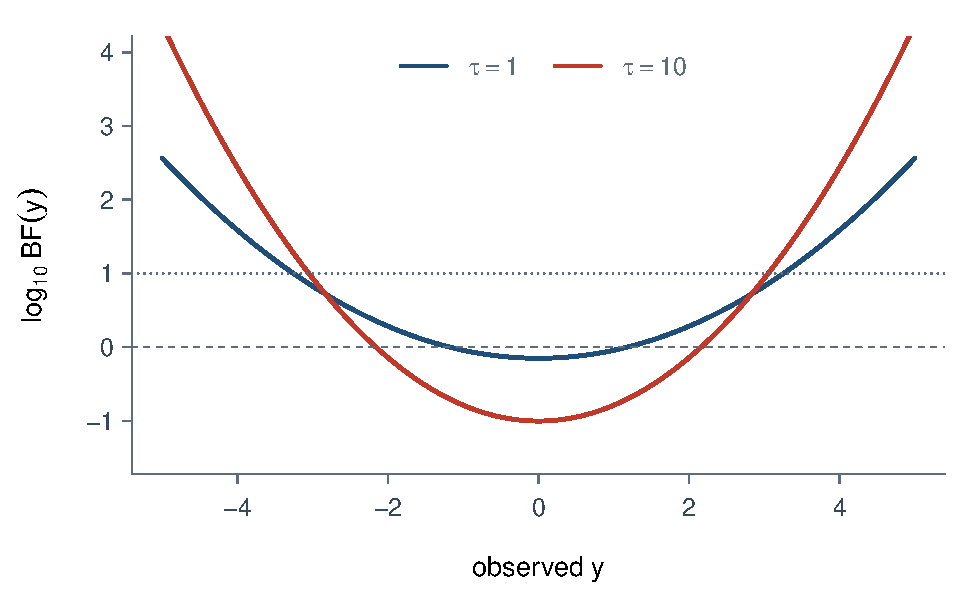
\includegraphics[width=0.72\linewidth]{ex05_bf.pdf}\end{center}
\step{(a) $\tau=1$.} $\text{BF}(0)=1/\sqrt2=0.71$ (data at 0 mildly favour $H_1$).
\begin{itemize}
\item BF $>1$ (posterior odds favour $H_2$): $|y|>1.18$.
\item BF $>10$ (strong evidence; our rejection rule): $|y|>3.26$.
\item BF $>100$ (decisive): $|y|>4.45$.
\end{itemize}
\step{(b) $\tau=10$.} $\text{BF}(0)=1/\sqrt{101}=0.10$ (data at 0 \emph{strongly} favour $H_1$).
\begin{itemize}
\item BF $>1$: $|y|>2.16$. \quad BF $>10$: $|y|>3.05$. \quad BF $>100$: $|y|>3.74$.
\end{itemize}

\step{Comments.}
\begin{itemize}
\item A vaguer alternative ($\tau=10$) needs a larger $|y|$ just to break even (2.16 vs.\ 1.18): it spreads its prior over a huge range and therefore predicts any particular moderate $y$ poorly.
\item But once $|y|$ is large, the BF grows faster for $\tau=10$ (its curve is steeper), because $\frac{\tau^2}{1+\tau^2}$ is closer to 1.
\item As $\tau\to\infty$, $\text{BF}(y)\to0$ for every fixed $y$ --- \textbf{Lindley's paradox}: an infinitely vague alternative can never win.
\end{itemize}

\begin{answer}
(a) $\tau=1$: reject $H_1$ (BF $>10$) when $|y|>3.26$ (BF $>1$ already for $|y|>1.18$). (b) $\tau=10$: reject when $|y|>3.05$ (BF $>1$ only for $|y|>2.16$). The vaguer prior penalises the alternative near $y=0$ but rises faster for large $|y|$; in the limit $\tau\to\infty$ the null always wins.
\end{answer}

\begin{takeaway}
For point-null tests, choose $\tau$ to reflect effect sizes you genuinely consider plausible --- never ``as large as possible''.
\end{takeaway}

% ================================================================= Exercise 6
\exercise{5.6 --- A/B/C testing for a mobile health app}

\begin{problem}{6}
You are on the design team for a mobile health app. Your team is considering three new designs labelled A, B and C. To identify the optimal design, $n=100$ users were randomly selected to be given each design and followed for a month. The table below gives the number of users in each treatment arm that opened the app $y$ times for $y$ between 0 and 6 (the maximum number of times the app was opened). For example, 100 users were given design A, and 40 of the 100 opened the app exactly once.
\begin{center}
\begin{tabular}{l|ccccccc|c}\toprule
Design & 0 & 1 & 2 & 3 & 4 & 5 & 6 & Total\\\midrule
A & 37 & 40 & 15 & 7 & 1 & 0 & 0 & 100\\
B & 12 & 29 & 28 & 16 & 8 & 6 & 1 & 100\\
C & 27 & 49 & 18 & 5 & 0 & 1 & 0 & 100\\\bottomrule
\end{tabular}
\end{center}
\begin{enumerate}[(a)]
\item Assuming the observations are Poisson counts, specify a likelihood and an objective Bayesian prior.
\item Perform an A/B test. Plot the posterior distribution of the Poisson rate parameter (i.e., the mean response) for each group, and compute the posterior probability that each of the three designs is optimal.
\end{enumerate}
\end{problem}

\begin{restate}
Which app design gets opened most often? Estimate each design's mean number of opens and the probability that each is the best.
\end{restate}

\begin{recall}
Poisson with Jeffreys prior (Exercise 2.19): $\pi(\lambda)\propto\lambda^{-1/2}$ $\Rightarrow$ $\lambda\mid\mathbf Y\sim\dist{Gamma}(\sum Y_i+\frac12,\ n)$.
\end{recall}

\begin{keyidea}
Only the total number of opens per design matters. ``Design $g$ is optimal'' = ``$\lambda_g$ is the largest''; its probability is the fraction of joint posterior draws in which $\lambda_g$ wins.
\end{keyidea}

\solution
\step{(a) Likelihood and prior.} For user $i$ with design $g$: $Y_{gi}\mid\lambda_g\iid\dist{Poisson}(\lambda_g)$; independent Jeffreys priors $\pi(\lambda_g)\propto\lambda_g^{-1/2}$ (objective and invariant to reparameterisation).
\step{(b) Step 1 --- totals.} A: $0\cdot37+1\cdot40+2\cdot15+3\cdot7+4\cdot1=95$; B: $29+56+48+32+30+6=201$; C: $49+36+15+0+5=105$.
\step{(b) Step 2 --- posteriors.} $\lambda_A\sim\dist{Gamma}(95.5,100)$, $\lambda_B\sim\dist{Gamma}(201.5,100)$, $\lambda_C\sim\dist{Gamma}(105.5,100)$.
\begin{center}
\begin{tabular}{lcc}\toprule
Design & Posterior mean & 95\% interval\\\midrule
A & 0.955 & (0.773, 1.156)\\
B & 2.015 & (1.746, 2.303)\\
C & 1.055 & (0.864, 1.266)\\\bottomrule
\end{tabular}
\end{center}
\begin{center}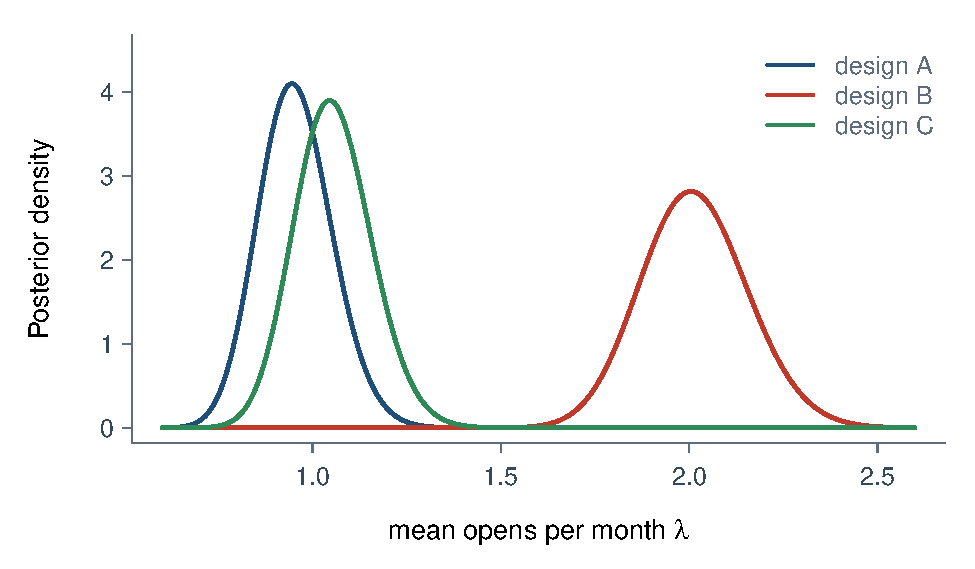
\includegraphics[width=0.7\linewidth]{ex06_rates.pdf}\end{center}
\step{(b) Step 3 --- probability each design is optimal} ($10^6$ joint draws): $\Prob(\text{A best})<10^{-6}$, $\Prob(\textbf{B best})\approx1$, $\Prob(\text{C best})<10^{-6}$. (Between the other two, C beats A with probability $\approx0.76$.)

\begin{sanity}
Is the Poisson assumption reasonable? Variance/mean ratios are A 0.94, B 0.98, C 0.78 --- close to 1, so yes (C is slightly under-dispersed). \checkmark
\end{sanity}

\begin{answer}
(a) $Y_{gi}\iid\dist{Poisson}(\lambda_g)$ with Jeffreys priors $\pi(\lambda_g)\propto\lambda_g^{-1/2}$. (b) Posterior means: A 0.96, B 2.02, C 1.06 opens per month; design B is optimal with posterior probability $\approx1$.
\end{answer}

\begin{takeaway}
``Probability of being the best'' is the quantity that drives Bayesian bandit algorithms (Section 5.3): future users would be sent mostly to design B.
\end{takeaway}

% ================================================================= Exercise 7
\exercise{5.7 --- Thyroid cancer hot spots and the Bayesian false discovery rate}

\begin{problem}{7}
The national average rate of new thyroid cancer cases is around 13 per 100,000 people. An epidemiological study is monitoring certain regions for rates exceeding the national rate. The population size ($N$) and the number of new cases ($Y$) for each region for the most recent year are:
\begin{center}
\small
\begin{tabular}{ccc|ccc}\toprule
Region & $N$ & $Y$ & Region & $N$ & $Y$\\\midrule
1 & 179611 & 20 & 11 & 30557 & 5\\
2 & 125453 & 18 & 12 & 81858 & 15\\
3 & 41646 & 7 & 13 & 103475 & 12\\
4 & 98826 & 22 & 14 & 166203 & 14\\
5 & 68642 & 10 & 15 & 52032 & 12\\
6 & 71844 & 6 & 16 & 85767 & 15\\
7 & 67702 & 9 & 17 & 145591 & 20\\
8 & 45954 & 9 & 18 & 139176 & 15\\
9 & 96325 & 18 & 19 & 87842 & 24\\
10 & 200201 & 27 & 20 & 97930 & 11\\\bottomrule
\end{tabular}
\end{center}
Separately for each region $i$, fit the model $Y_i|\lambda_i\sim\dist{Poisson}(N_i\lambda_i)$ with prior $\lambda_i\sim\dist{Gamma}(a,b)$, and compute the posterior probability that the region's rate $\lambda_i$ exceeds the national average $\lambda_0=13/100000$, denoted $q_i=\Prob(\lambda_i>\lambda_0|Y_i)$.
\begin{enumerate}[(a)]
\item Select $a$ and $b$ so that (approximately) the prior probability that $\lambda_1>\lambda_0$ is 0.5, and the prior 0.95 quantile is $10\lambda_0$.
\item Assuming that you will conclude the rate in region $i$ exceeds the national average if $q_i>t$, select $t$ to control the Bayesian false discovery rate at 10\%. With this value, summarize the results.
\end{enumerate}
\end{problem}

\begin{restate}
For each of 20 regions, compute the probability that its cancer rate exceeds the national rate; then choose a cut-off so that, on average, at most 10\% of the regions we flag are false alarms.
\end{restate}

\begin{recall}
\begin{itemize}
\item Gamma scaling: quantiles of $\dist{Gamma}(a,b)$ are $\dist{Gamma}(a,1)$ quantiles divided by $b$, so the \emph{ratio} of two quantiles depends only on $a$.
\item Bayesian FDR: primer, point 5.
\end{itemize}
\end{recall}

\begin{keyidea}
(a) Two conditions: median $=\lambda_0$ and 95th percentile $=10\lambda_0$. The ratio $q_{0.95}/q_{0.5}=10$ fixes $a$; then the median fixes $b$. (b) Rank the regions by $q_i$ and flag from the top until the average of $1-q_i$ among flagged regions would exceed 0.10.
\end{keyidea}

\solution
\step{(a) Step 1 --- the shape $a$.} Solve $\frac{\texttt{qgamma(0.95, a, 1)}}{\texttt{qgamma(0.5, a, 1)}}=10$ numerically: $a=0.4395$.
\step{(a) Step 2 --- the rate $b$.} $b=\frac{\texttt{qgamma(0.5, a, 1)}}{\lambda_0}=1359.4$. Check: $\Prob(\lambda>\lambda_0)=0.500$ and $q_{0.95}=10.00\lambda_0$. \checkmark
\why{The prior is centred on the national rate but allows rates up to 10 times higher: a weakly informative, sceptical prior.}

\step{(a) Step 3 --- $q_i$ for each region.} $\lambda_i\mid Y_i\sim\dist{Gamma}(0.4395+Y_i,\ 1359.4+N_i)$, $q_i=\Prob(\lambda_i>\lambda_0\mid Y_i)$. Sorted by $q_i$ (rates per 100{,}000):
\begin{center}
\small
\begin{tabular}{ccccc|ccccc}\toprule
Region & $Y/N$ & post.\ mean & $q_i$ & flagged & Region & $Y/N$ & post.\ mean & $q_i$ & flagged\\\midrule
19 & 27.3 & 27.4 & 0.9993 & \checkmark & 2 & 14.3 & 14.5 & 0.6531 & \\
4 & 22.3 & 22.4 & 0.9890 & \checkmark & 5 & 14.6 & 14.9 & 0.6290 & \\
15 & 23.1 & 23.3 & 0.9622 & \checkmark & 17 & 13.7 & 13.9 & 0.5902 & \\
9 & 18.7 & 18.9 & 0.9234 & \checkmark & 10 & 13.5 & 13.6 & 0.5698 & \\
12 & 18.3 & 18.6 & 0.8911 & \checkmark & 7 & 13.3 & 13.7 & 0.5174 & \\
8 & 19.6 & 20.0 & 0.8678 & \checkmark & 13 & 11.6 & 11.9 & 0.3369 & \\
16 & 17.5 & 17.7 & 0.8578 & \checkmark & 20 & 11.2 & 11.5 & 0.3034 & \\
3 & 16.8 & 17.3 & 0.7319 & \checkmark & 1 & 11.1 & 11.3 & 0.2345 & \\
11 & 16.4 & 17.0 & 0.6765 & & 18 & 10.8 & 11.0 & 0.2224 & \\
 & & & & & 6, 14 & 8.4 & 8.6--8.8 & $\le0.12$ & \\\bottomrule
\end{tabular}
\end{center}

\step{(b) Choosing $t$.}
\begin{center}
\begin{tabular}{cccccc}\toprule
Flag top & 6 & 7 & \textbf{8} & 9 & 10\\\midrule
threshold $t$ & 0.858 & 0.732 & \textbf{0.677} & 0.653 & 0.629\\
BFDR & 0.061 & 0.073 & \textbf{0.097} & 0.122 & 0.145\\\bottomrule
\end{tabular}
\end{center}
\why{Example: flagging the top 8 regions, $\text{BFDR}=\frac{(1-0.9993)+(1-0.9890)+\dots+(1-0.7319)}{8}=0.097\le0.10$; adding region 11 ($q=0.677$) would raise it to 0.122.}
So $t=0.677$ (flag regions with $q_i>0.677$).

\begin{answer}
(a) $\lambda\sim\dist{Gamma}(0.44,\ 1359)$. (b) $t=0.677$ controls the BFDR at 9.7\%. Eight regions are flagged as exceeding the national rate: 19, 4, 15, 9, 12, 8, 16 and 3 (in decreasing order of evidence). Regions 19 and 4 (about 27 and 22 cases per 100{,}000) are nearly certain hot spots; for the others the evidence is moderate, and we expect less than one of the eight to be a false alarm.
\end{answer}

\begin{takeaway}
Controlling the FDR accepts a few false alarms in exchange for power --- appropriate for screening, where flagged regions are followed up anyway.
\end{takeaway}

% ================================================================= Exercise 8
\exercise{5.8 --- Frequentist properties of a Bayesian test}

\begin{problem}{8}
Assume the model $Y_i|\lambda\sim\dist{Poisson}(\lambda)$ for $i=1,\dots,n$ and improper prior $\pi(\lambda)\propto1$. The objective is to test the null hypothesis $H_1:\lambda\le1$ versus the alternative hypothesis $H_2:\lambda>1$, and the test is to reject the null hypothesis if $\Prob(\lambda>1|Y_1,\dots,Y_n)>0.95$.
\begin{enumerate}[(a)]
\item Assuming $n$ is fixed at 10, compute the probability of rejecting the null hypothesis for true $\lambda$ ranging from 1 to 2.
\item Assuming the true value of $\lambda$ is 1, compute the Type I error of the test for $n$ ranging from 10 to 100.
\item Assuming the true value of $\lambda$ is 1.5, compute the power of the test for $n$ ranging from 10 to 100.
\item How might you modify the test to guarantee that the Type I error is exactly 0.05?
\end{enumerate}
\end{problem}

\begin{restate}
Study how often the Bayesian rule ``reject if $\Prob(\lambda>1\mid\text{data})>0.95$'' rejects in repeated samples, for different true $\lambda$ and sample sizes.
\end{restate}

\begin{recall}
\begin{itemize}
\item Flat prior + Poisson data: $\lambda\mid\mathbf Y\sim\dist{Gamma}(S+1,\ n)$ with $S=\sum Y_i$.
\item $S\sim\dist{Poisson}(n\lambda_{\text{true}})$ in repeated samples.
\end{itemize}
\end{recall}

\begin{keyidea}
The posterior depends on the data only through $S$, and $\Prob(\lambda>1\mid S)$ increases with $S$. So the rule is ``reject if $S\ge s_n$'' for a critical value $s_n$, and $\Prob(\text{reject})=\Prob(S\ge s_n)$ is an exact Poisson tail probability --- no simulation needed.
\end{keyidea}

\solution
\step{Step 1 --- the critical value.} For each $n$, $s_n$ is the smallest $s$ with \texttt{pgamma(1, s + 1, n, lower.tail = FALSE)} $>0.95$. For $n=10$: $s_{10}=15$.
\step{(a) $n=10$.} $\Prob(\text{reject}\mid\lambda)=\Prob\big(\dist{Poisson}(10\lambda)\ge15\big)$:
\begin{center}
\begin{tabular}{c|cccccc}\toprule
true $\lambda$ & 1.0 & 1.2 & 1.4 & 1.6 & 1.8 & 2.0\\\midrule
$\Prob(\text{reject})$ & 0.084 & 0.228 & 0.430 & 0.633 & 0.792 & 0.895\\\bottomrule
\end{tabular}
\end{center}
\step{(b), (c) Type I error and power for $n=10,\dots,100$.}
\begin{center}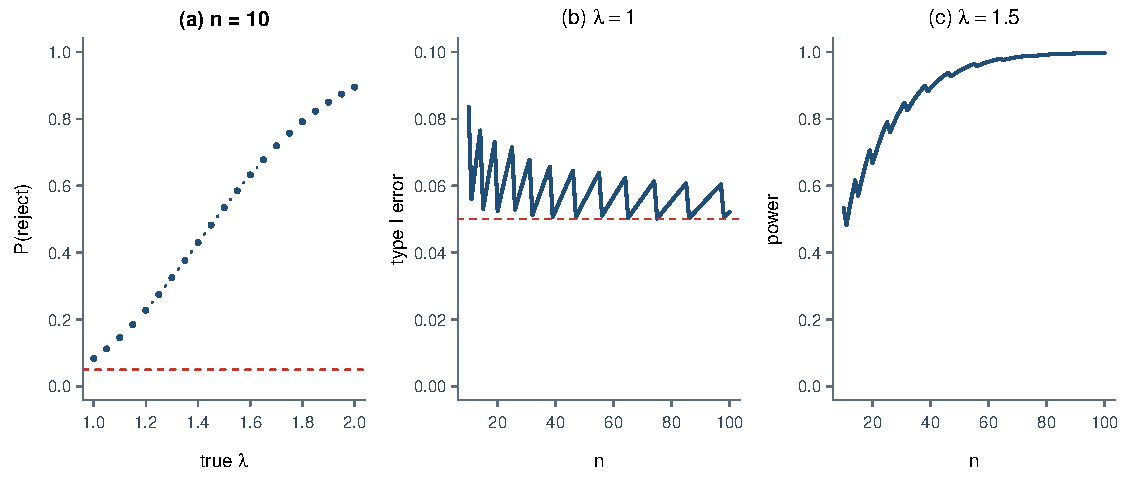
\includegraphics[width=0.98\linewidth]{ex08_power.pdf}\end{center}
Type I error ($\lambda=1$) ranges from 0.050 to 0.084 (average 0.058) --- \emph{always at least} 0.05, with a saw-tooth pattern because $S$ is discrete. Power at $\lambda=1.5$: 0.53 ($n=10$), 0.67 ($n=20$), 0.94 ($n=50$), 0.998 ($n=100$).
\why{Why is the type I error too big? The flat prior $\pi(\lambda)\propto1$ adds ``one extra event'' (posterior shape $S+1$), nudging the posterior upward, so the rule rejects slightly too easily. The effect fades as $n$ grows.}

\step{(d) Getting exactly 0.05.}
\begin{itemize}
\item \textbf{Calibrate the cut-off}: for each $n$, choose $s_n$ from the null distribution $S\sim\dist{Poisson}(n)$ rather than from the 0.95 posterior rule; because $S$ is discrete this gives type I error $\le0.05$, and
\item \textbf{randomise at the boundary}: reject if $S>s_n^*$, and reject with probability $\gamma$ if $S=s_n^*$, with $\gamma=\frac{0.05-\Prob(S>s_n^*)}{\Prob(S=s_n^*)}$. This makes the type I error exactly 0.05.
\end{itemize}
(Using the Jeffreys prior $\lambda^{-1/2}$ instead of the flat prior brings the error much closer to 0.05, but not exactly.)

\begin{answer}
(a) Rejection probability rises from 0.08 ($\lambda=1$) to 0.90 ($\lambda=2$). (b) Type I error 0.050--0.084, always above 0.05 (flat prior + discreteness). (c) Power at $\lambda=1.5$ grows from 0.53 ($n=10$) to 0.998 ($n=100$). (d) Calibrate the cut-off to the null distribution of $S$ and randomise at the boundary.
\end{answer}

\begin{takeaway}
Bayesian procedures can (and often should) be checked for their frequentist behaviour --- this is how sample sizes for Bayesian trials are planned (Section 5.4).
\end{takeaway}

% ================================================================= Exercise 9
\exercise{5.9 --- Stochastic search variable selection for Boston housing}

\begin{problem}{9}
Download the Boston Housing Data in R from the Boston dataset. The response is medv, the median value of owner-occupied homes, and the other 13 variables are covariates that describe the neighborhood. Use stochastic search variable selection (SSVS) to compute the most likely subset of the 13 covariates to include in the model and the marginal probability that each variable is included in the model. Clearly describe the model you fit including all prior distributions.
\end{problem}

\begin{restate}
Which of the 13 neighbourhood variables really belong in the regression for house values? Use SSVS to get each variable's inclusion probability and the best subset.
\end{restate}

\begin{recall}
\textbf{Collapsed SSVS.} With a conjugate prior the regression coefficients can be integrated out, leaving the marginal likelihood $m(\mathbf Y\mid\bm\gamma)$ of each subset $\bm\gamma$ in closed form. The Gibbs sampler then updates each $\gamma_j$ from
\[
\Prob(\gamma_j=1\mid\bm\gamma_{-j},\mathbf Y)=\frac{m(\mathbf Y\mid\gamma_j=1,\bm\gamma_{-j})}{m(\mathbf Y\mid\gamma_j=1,\bm\gamma_{-j})+m(\mathbf Y\mid\gamma_j=0,\bm\gamma_{-j})}\quad(\text{prior }\gamma_j\sim\dist{Bernoulli}(0.5)).
\]
\end{recall}

\begin{keyidea}
With only $2^{13}=8{,}192$ possible subsets we can also compute the \emph{exact} posterior of every model and check the SSVS sampler against it.
\end{keyidea}

\solution
\step{Model and priors.}
\[
\text{medv}_i=\beta_0+\sum_{j=1}^{13}\gamma_j\beta_jZ_{ij}+\varepsilon_i,\qquad\varepsilon_i\iid\dist N(0,\sigma^2),
\]
with $Z_{ij}$ the standardised covariates and
\[
\pi(\beta_0)\propto1,\qquad\beta_j\mid\sigma^2\iid\dist N(0,\ W\sigma^2)\ (W=1),\qquad\pi(\sigma^2)\propto1/\sigma^2,\qquad\gamma_j\iid\dist{Bernoulli}(0.5).
\]
\why{$W=1$ says an included variable's effect (per SD) is typically of the order of the noise SD ($\approx\$4{,}700$) --- realistic for house prices; $\gamma_j\sim\dist{Bernoulli}(0.5)$ makes all $8{,}192$ subsets equally likely a priori.}
\step{Marginal likelihood of a subset.} Integrating out $\beta_0$, $\bm\beta_\gamma$ and $\sigma^2$ (centred $\tilde{\mathbf y}$, $k=\sum\gamma_j$, $\mathbf A=\mathbf Z_\gamma^\top\mathbf Z_\gamma+\mathbf I/W$):
\[
\log m(\mathbf Y\mid\bm\gamma)=-\tfrac k2\log W-\tfrac12\log|\mathbf A|-\tfrac{n-1}{2}\log\big(\tilde{\mathbf y}^\top\tilde{\mathbf y}-\tilde{\mathbf y}^\top\mathbf Z_\gamma\mathbf A^{-1}\mathbf Z_\gamma^\top\tilde{\mathbf y}\big)+\text{const}.
\]
\step{SSVS sampler.} 6{,}000 sweeps (1{,}000 burn-in), each updating all 13 $\gamma_j$ in random order.
\begin{center}
\begin{tabular}{lcc|lcc}\toprule
Variable & SSVS & exact & Variable & SSVS & exact\\\midrule
crim & 0.925 & 0.924 & dis & 1.000 & 1.000\\
zn & 0.935 & 0.937 & rad & 0.993 & 0.992\\
indus & \textbf{0.089} & 0.087 & tax & 0.963 & 0.964\\
chas & 0.892 & 0.891 & ptratio & 1.000 & 1.000\\
nox & 1.000 & 1.000 & black & 0.968 & 0.961\\
rm & 1.000 & 1.000 & lstat & 1.000 & 1.000\\
age & \textbf{0.075} & 0.073 & & & \\\bottomrule
\end{tabular}
\end{center}
\begin{center}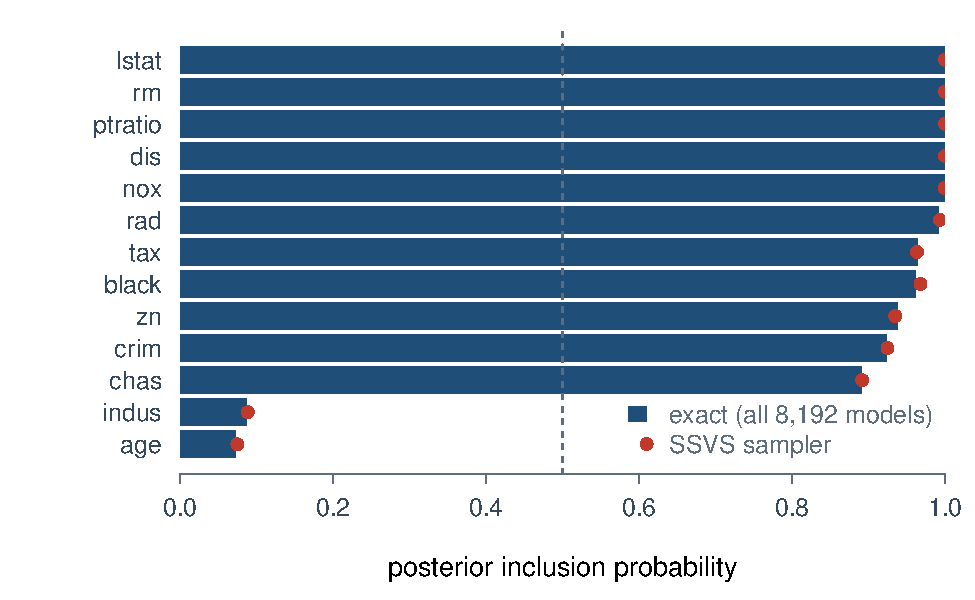
\includegraphics[width=0.75\linewidth]{ex09_inclusion.pdf}\end{center}
\step{Most likely subsets.}
\begin{center}
\small
\begin{tabular}{cl}\toprule
Posterior prob. & Model\\\midrule
\textbf{0.615} & all except \texttt{indus} and \texttt{age}\\
0.079 & all except \texttt{indus}, \texttt{age} and \texttt{chas}\\
0.056 & all except \texttt{age}\\
0.048 & all except \texttt{indus}\\
0.045 & all except \texttt{indus}, \texttt{age} and \texttt{crim}\\\bottomrule
\end{tabular}
\end{center}

\begin{sanity}
The SSVS chain visits the top model 61.8\% of the time, matching its exact posterior probability 0.615, and every inclusion probability agrees with the exact enumeration to within 0.007. \checkmark
\end{sanity}

\begin{answer}
Model: standardised linear regression with $\beta_j\mid\sigma^2\sim\dist N(0,\sigma^2)$ for included variables, flat intercept, $\pi(\sigma^2)\propto1/\sigma^2$, $\gamma_j\sim\dist{Bernoulli}(0.5)$. The most likely subset (posterior probability 0.62) contains all variables except \texttt{indus} and \texttt{age}. Inclusion probabilities: \texttt{indus} 0.09, \texttt{age} 0.07, \texttt{chas} 0.89, \texttt{crim} 0.92, \texttt{zn} 0.94, \texttt{tax} 0.96, \texttt{black} 0.96, the rest $\ge0.99$.
\end{answer}

\begin{takeaway}
This agrees with Exercise 4.2: \texttt{indus} and \texttt{age} were exactly the coefficients whose intervals contained 0 and which the LASSO prior shrank to zero.
\end{takeaway}

\end{document}
